\documentclass[12pt]{report}

\usepackage[utf8]{inputenc}
\usepackage[T1]{fontenc}
\usepackage{graphicx}
\usepackage[french]{babel} 
\usepackage[top=3cm, bottom=3cm, left=3cm, right=3cm]{geometry}
\usepackage{tikz}
\usepackage{color}
\usepackage{colortbl}
\usepackage[colorlinks=true,linktocpage]{hyperref}
\usepackage{hyperref}
\usepackage{listings}
\usepackage{amsmath}
\usepackage{diagbox}
\usepackage{framed}
\usepackage{float}
\usepackage{amsmath}
\usepackage{amssymb}

\definecolor{mygray}{rgb}{0.5,0.5,0.5}
\lstdefinestyle{CLangage}{
language=C,
basicstyle=\normalsize,
backgroundcolor=\color[rgb]{0.95,0.95,0.95},
upquote=true,
xleftmargin=30pt,
framexleftmargin=13pt,
        framextopmargin=3pt,
        framexbottommargin=3pt, 
        frame=tb, framerule=0pt,
aboveskip={0.2\baselineskip},
showstringspaces=true,
extendedchars=true,
breaklines=true,
showtabs=false,
showspaces=false,
showstringspaces=false,
identifierstyle=\ttfamily,
keywordstyle=\color[rgb]{0,0,1},
commentstyle=\footnotesize\color[rgb]{0.133,0.545,0.133},
stringstyle=\color[rgb]{0.627,0.126,0.941},
numbers=left,                    % where to put the line-numbers; possible values are (none, left, right)
  numbersep=5pt,
   numberstyle=\tiny\color{mygray},
   stepnumber=1,
   morekeywords={X:,T:,C:,M:,L:,Q:,K:,V:},
}
\lstdefinestyle{Bash}{
language=Bash,
basicstyle=\normalsize,
backgroundcolor=\color[rgb]{0.95,0.95,0.95},
upquote=true,
xleftmargin=30pt,
framexleftmargin=13pt,
        framextopmargin=3pt,
        framexbottommargin=3pt, 
        frame=tb, framerule=0pt,
aboveskip={0.2\baselineskip},
columns=fullflexible,
showstringspaces=true,
extendedchars=true,
breaklines=true,
showtabs=false,
showspaces=false,
showstringspaces=false,
identifierstyle=\ttfamily,
keywordstyle=\color[rgb]{0,0,1},
commentstyle=\footnotesize\color[rgb]{0.133,0.545,0.133},
stringstyle=\color[rgb]{0.627,0.126,0.941},
numbers=none,                    % where to put the line-numbers; possible values are (none, left, right)
  numbersep=5pt,
   numberstyle=\tiny\color{mygray},
   stepnumber=1
}
\definecolor{grey}{rgb}{0.95, 0.95, 0.95}


\begin{document}

\title{\begin{Huge}Editeur musical avec lecture audio\end{Huge} \\
    \begin{normalsize}\textit{et génération analogique d'ondes sinusoidales et carrées}\end{normalsize}
    }
\author{Victor \bsc{Veillerette}}
\date{Janvier 2017}
 
\maketitle

\tableofcontents

\addtocontents{toc}{\protect\enlargethispage{\baselineskip\baselineskip\baselineskip}}
\chapter{Introduction}
\section{Sujet initial}
\section{Analyse des fonctionnalités} % midi -> dur d'implémentation, pour plus tard ?

\chapter{Développement} % Sources, Organisation dossiers, Bibliothèques, Histogramme ?
\section{Sources}
Le projet est une application entièrement écrite en C ANSI (1989). 
Il est à noter que le programme n'utilise aucune image externe et génère de lui-même tous les dessins affichés à l'écran. Pour cela le programme utilise les librairies suivantes :\\
\begin{itemize}
 \item \textbf{SDL-1.2} : La librairie \textit{Simple Direct Media Library} permet l'ouverture d'une fenêtre, le remplissage de rectangles, la gestion des événements.\\
 \item \textbf{SDL\_gfx 2.0.25} : Cette extension de la SDL permet l'utilisation de primitives de dessin et de zoom plus évoluées.\\
 \item \textbf{SDL\_ttf 2.0} : Cette extension de la SDL permet l'affichage de texte à l'écran. \\
\end{itemize}
 Le dossier principal du projet est organisé de la façon suivante :\\
\begin{itemize}
 \item \textbf{doxygen/} : Documentation technique générée par Doxygen. Elle regroupe la documentation complète de toutes les structures et de toutes les fonctions du projet.\\
 \item \textbf{media/} : Fichiers de polices nécessaires à l'exécution de l'application.\\
 \item \textbf{include/} : Fichiers headers du projet .h; chaque fichier est rattaché à un fichier source, et donc à un module.\\
 \item \textbf{doc/} : Quelques fichiers exemples .abc ou .med à charger dans l'application.\\
 \item \textbf{src/} : Fichiers sources du projet .c; chaque fichier correspond à un module. \\
 \item \textbf{Makefile} : Fichier Makefile permettant la compilation simple avec la commande \textit{make}\\
 \item \textbf{Rapport.pdf} : Ce même rapport. \\
\end{itemize}
\section{Plateforme de suivi Git}
Malgré le fait que le développement du programme ne soit effectué que par une personne, j'ai voulu tester l'utilisation du logiciel de gestion de version \textbf{git}
avec la plateforme en ligne \textbf{Github.com}\footnote{\url{https://github.com/}}.\\ \\
Le projet est constitué d'environ 110 commits pour plus de 10000 lignes :\\

\begin{figure}[H]
  \centering
  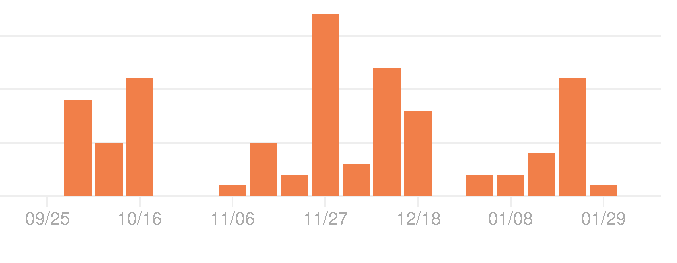
\includegraphics[scale=0.58]{git2.png}\\
    \caption{\textit{Evolution du nombre de commits par semaine}}
\end{figure}


\chapter{Implémentations}
\section{Partition}
\subsection{Durée des notes}
La durée des notes est représentée dans le programme comme dans le domaine de la notation musicale, c'est-à-dire qu'une Ronde se note 1, une Blanche 2, une Noire 4, etc.\\
Sachant que le programme représente les durées de base de la Ronde jusqu'à la Quadruple-Croche, il est alors possible de récupérer la durée réelle d'une note grâce à la formule :\\
\[ Real\_Duration(duration) = \frac{64}{duration} \]\\
\lstset{style=CLangage}
\begin{lstlisting}[language=C]
typedef enum {
	RONDE = 1,		BLANCHE	= 2,
	NOIRE = 4,		CROCHE	= 8,
	DOUBLECROCHE = 16, 	TRIPLECROCHE = 32
	QUADRUPLECROCHE = 64
	} Note_Duration;
\end{lstlisting}
\newpage
\subsection{Hauteur des notes}
La hauteur des notes suit la spécification MIDI mais commence à l'octave 0 jusqu'à la fin de l'octave 8 : \\
\begin{center}
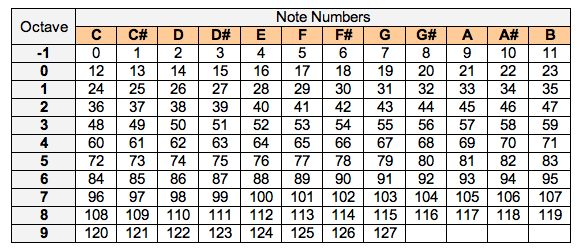
\includegraphics[scale=0.50]{midi.jpg}
\end{center}
\vskip 0.3in
\subsection{Structure d'une note}
Une note est représentée par sa hauteur, sa durée, des drapeaux (Altérations, note pointée, liaison). Ici un silence est représenté de la même manière
(certains champs sont alors ignorés). La structure suivante d'une note combinant ces deux aspects est donc utilisée :\\
\lstset{style=CLangage}
\begin{lstlisting}[language=C]
struct Note
{
	char note; 	/* Hauteur */
	char rest; 	/* Note / Silence */
	
	Note_Flags flags : 24;	/* Drapeaux */
	Note_Duration duration : 8;	/* Duree */
};
\end{lstlisting}
\subsection{Représentation d'une mesure}
Une mesure est représentée par un type de mesure (4/4, 3/4 , ...), une clé, des drapeaux, une armure et une suite de note structurée
comme une liste chaînée simple.\\Au départ, une mesure est initialisée avec uniquement des silences (les plus grands possibles).\\ La durée totale
de la mesure (num * den) est conservée à l'ajout et à la suppression de note (qui équivaut à changer le champ rest d'une note).\\ \newpage
Voici la structure pour représenter une mesure :\\
\lstset{style=CLangage}
\begin{lstlisting}[language=C]
struct Step
{
	ToNote *notes;		/* Liste chainees */
	int num;		/* Nombre de temps */
	Cle cle : 16;		/* Cle */
	Note_Duration den : 8;	/* Duree de base */
	Step_Flags flags : 16;	/* Drapeaux */
	signed char sign;	/* Armure */
};
\end{lstlisting}
\vskip 0.3in
L'armure est constituée comme ceci :\\
\begin{itemize}
 \item Si \textbf{sign} vaut 0, alors la tonalité est de DoM/Lam : l'armure est vide.\\
 \item Si \textbf{sign} est négatif, alors l'armure est constituée de |sign| bémols.\\
 \item Si \textbf{sign} est positif, alors l'armure est constituée de sign dièses.\\
\end{itemize}

\subsection{Portée et Partition}
Une portée n'est qu'un tableau de plusieurs mesures les unes à la suite des autres. En effet, la suppression/déplacement d'une mesure est une
opération coûteuse en performance mais rare dans cette utilisation.\\
De la même manière, une partition est un tableau de plusieurs portées. Il est à noter qu'il est évident que chaque portée doit avoir le même nombre
de mesures : Ceci est vérifié par les fonctions d'ajouts/suppressions de mesures qui permettent de garder cet état vrai.\\

\newpage
\section{Audio}
\subsection{Principe}
Il est à noter qu'ici, en aucun cas le programme n'utilise la librairie SDL\_mixer qui faciliterait l'utilisation de
sons MP3/WAV externes mais qui empêcherait la configuration des fréquences jouées.\\
Le programme travaille avec des signaux de caractéristiques suivantes :\\
\begin{itemize}
 \item \textbf{Un taux d'échantillonage} de 44100Hz (qualité CD) : Une seconde d'un signal audio est divisée en 44100 valeurs.\\
 \item des valeurs en \textbf{16 bits signés} \\
 \item \textbf{2 Channels} (Gauche / Droite)\\
 \item Un buffer audio \textbf{de 256 valeurs}. \\
\end{itemize}

\subsection{Fréquences de base}
Pour calculer la fréquence de base d'une note dans la gamme tempérée, le programme utilise la formule suivante :\\
\begin{large}
\[ 
  f(h) = 33 \times {2}^{(\frac{h}{12} - 2)} \times {1.059463}^{(h \bmod 12)}
\]
\end{large}

\subsection{Remplissage du buffer et Mixage}
La fonction \textbf{main\_callback()} du fichier Audio.c se charge de remplir le buffer une fois que celui-ci est vide.\\ \\
Dans un premier temps, cette fonction va faire appel à une fonction de mixage.\\ Celle-ci va considérer toutes les notes
jouées en cours et additionner leur signal et normaliser le signal résultant.\\ \\ Ce signal de 256 valeurs va ensuite être
copié dans le buffer pour être joué.\\\\
Voici comment calculer un signal à partir d'une fréquence :\\

\begin{figure}[H]
\centering
\[
\begin{aligned}
sinusoide(x, frequence) &  =  \sin(\pi\times \mathit{frequence}\times \frac{x}{44100}) \\
carre(x, frequence)  & =   \lfloor sinusoide(x, \mathit{frequence}) \rfloor   \\
fusion(x, frequence) & =  \mathit{carre}(x, \mathit{frequence}) + \mathit{sinusoide}(x, \mathit{frequence})  \\
harmo(x, frequence) & =  \sum_{i=0}^{4} \mathit{carre}(x, \mathit{frequence}\times 2^i)
\end{aligned}
 \]
\caption{\textit{Génération des signaux}}
\end{figure}



\subsection{Lecture}
Un thread est créé pour chaque portée. Ainsi, chaque thread va analyser la mesure suivant, trouver la note à jouer et l'envoyer au mixeur du processus parent.\\
Les threads utilisés sont les SDL\_Thread gérés automatiquement par la librairie.\\


\newpage
\chapter{Eléments Techniques}
\section{Compilation et Lancement}
Pour compiler le projet, un Makefile est fourni. Il créera le programme \textbf{med}. Pour lancer la compilation, 
il suffit de lancer la commande \textbf{make} et pour retourner à un dossier propre, d'utiliser la commande \textbf{make clean},
ce qui supprimera l'exécutable et les fichiers temporaires liés à la compilation :\\
\lstset{style=Bash}
\begin{lstlisting}
make 		   #Compilation
make clean 	   #Nettoyage
\end{lstlisting}
\vskip 0.1in
Pour lancer l'application il suffit d'exécuter le programme qui vient d'être compilé. Il est aussi possible d'importer un fichier MED ou ABC directement en ligne de commande :\\
\begin{lstlisting}
./med #Lancement simple
./med file.med     #Lancement avec ouverture du fichier MED file.med
./med -abc file.abc  #Lancement avec importation du fichier ABC file.abc
\end{lstlisting}

\section{Format MED}
Le format MED est le format propre du projet. C'est un format binaire qui se base sur la recopie octet par octet de la mémoire dans un fichier. Cela permet une sauvegarde et une ouverture rapide.\\
Ce format est un fichier non compressé, il est donc relativement lourd (quelques ko à 5-6Mo en fonction de la taille de la partition) puisque la plupart des octets du fichier sont à 0 et que le programme
autorise la redondance d'informations en mémoire. \\

\section{Format ABC}
Le programme permet d'importer ou d'exporter des fichiers au format ABC. Étant donné que c'est un format très libre et très permissif, 
seul le format ABC 2.0\footnote{Documentation ABC 2.0 : \url{http://abcnotation.com/wiki/abc:standard:v2.0}} peut être importé. Mais vu qu'il n'y a pas moyen de différencier les versions,
le programme tentera quand même d'ouvrir tout type de fichier ABC.\\ \\
Toutefois, toutes les fonctionnalités ne sont pas supportées et le programme commence par modifier la syntaxe du fichier en entrée (simplification et création d'un nouveau fichier temporaire),
puis il tente de le parser.\\\\
Voici le format idéal reconnu :\\\vskip 0.3in
Le format se compose d'abord d'un header: \\
\begin{lstlisting}[language=Tex]
X:7959		     % Identifiant unique de melodie (obligatoire)
T:Titre		     % Titre
C:Compositeur	     % Compositeur
M:3/4		     % Mesure
L:1/8		     % Duree de base pour une note
Q:1/4=90 	     % Tempo
K:F		     % Tonalite
\end{lstlisting}\vskip 0.3in
Puis le corps du format avec les informations sur les notes :\\
\begin{lstlisting}[language=Tex]
V:1	  	 % Numero de voix (1 = 1ere voix)
c f2 a/ g/ g/ f/ e/ f/ | c g2 b/ a/ a/ g/ ^f/ g/ |
V:2		 % Numero de voix (2 = 2eme voix)
F, C F, C F, C | E, C E, C E, C |
\end{lstlisting}
\vskip 0.6in
\newpage
Voici quelques significations des symboles présentés ci-dessus et qui peuvent être retrouvées dans la documentation :

\def\arraystretch{1.5}

\begin{center}
\begin{tabular}{>{\columncolor{grey}} c <{}|ccc}
\hline


\rowcolor{grey}\textbf{Symbole} & \textbf{Signification}\\

\hline


abcdefg & Nom des notes \\ \hline
ABCDEFG & Nom des notes un octave plus bas \\ \hline
|	& Séparation des mesures \\ \hline
z ou x	& Silence \\ \hline
V\string:chiffre & Numéro de voix de la prochaine ligne (maximum 10) \\ \hline
/[nombre] & Divise la durée de base de la note \\ \hline
[nombre] & Multiplie la durée de base de la note \\ \hline
,	& Diminue d'un octave \\ \hline
'	& Augmente d'un octave \\ \hline
\textasciicircum	& Ajout d'un dièse sur la prochaine note \\ \hline
=	& Ajout d'un bécarre sur la prochaine note \\ \hline
\_	& Ajout d'un bémol sur la prochaine note \\ \hline

\end{tabular}
\end{center}
\vskip 0.6in

\section{Bugs connus}
Voici en vrac, dans un ordre non particulier, une liste de bugs, de comportements non souhaités ou de fonctionnalités non mis en place :\\
\begin{itemize}
 \item Problème d'importation des fichiers ABC écrits sous Windows/Mac avec le retour à la ligne \textbf{\textbackslash r\textbackslash n} ou \textbf{\textbackslash r}. \\
 \item ... Bla ... Bla
\end{itemize}

\chapter{Manuel d'utilisation}
\section{Interface générale}


\section{Explorateur de fichier}
\section{Configuration Audio}

\chapter{Bilan}
\section{Conclusion}
\section{Perspectives} % Imporation/Export fichier MIDI, Compression format .med (Huffman...), 
\end{document}
